% =====================================================================
%  Chapitre 9 : Formulaires
% =====================================================================
\chapter{Les formulaires Django}
\label{ch:formulaires}

\chapitreresume{Un catalogue sans saisie serait bien triste. Dans ce chapitre, vous
créez des formulaires capables de valider les données, de téléverser une couverture
et d'enregistrer un emprunt. Vous découvrez \code{forms.Form}, \code{ModelForm}, la
validation personnalisée, les messages et les vues de création, de modification et
de suppression.}

\begin{objectifs}
\begin{itemize}
  \item Distinguer un formulaire HTML d'un formulaire Django.
  \item Écrire un \code{forms.Form} et un \code{ModelForm}.
  \item Afficher un formulaire dans un gabarit et gérer les erreurs.
  \item Traiter une requête \code{POST} avec \code{csrf\_token}.
  \item Valider un emprunt avec \code{clean()} et \code{clean\_<champ>()}.
  \item Téléverser une image de couverture.
  \item Afficher des messages flash après une action.
  \item Écrire les vues de création, de modification et de suppression.
  \item Découvrir \code{CreateView} et \code{UpdateView} en alternative.
\end{itemize}
\end{objectifs}

\section{Pourquoi un formulaire Django ?}

Un formulaire HTML envoie des chaînes. Il faut ensuite vérifier que le titre n'est
pas vide, que l'ISBN contient treize chiffres, que l'année est plausible, que
l'auteur existe. Django centralise ces vérifications dans une classe Python.

\begin{retenir}
Un formulaire Django fait trois choses : il génère le HTML, il valide les données et
il nettoie les valeurs. La vue n'a plus qu'à tester \code{form.is\_valid()} et à
enregistrer. C'est plus sûr et plus lisible qu'une série de \code{if} dans le
gabarit.
\end{retenir}

\section{Un premier formulaire}

\begin{codebox}[python]{catalogue/forms.py}
from django import forms


class ContactForm(forms.Form):
    nom = forms.CharField(
        max_length=80,
        label="Votre nom",
    )
    email = forms.EmailField(label="Votre adresse électronique")
    message = forms.CharField(
        label="Message",
        widget=forms.Textarea(attrs={"rows": 5}),
    )
    copie = forms.BooleanField(
        label="Recevoir une copie",
        required=False,
    )
\end{codebox}

\begin{description}[leftmargin=3.9cm,style=nextline]
  \item[\code{CharField}] Texte court. \code{max\_length} est obligatoire pour la
  validation.
  \item[\code{EmailField}] Vérifie le format de l'adresse.
  \item[\code{BooleanField}] Case à cocher. \code{required=False} la rend
  facultative.
  \item[\code{label}] Texte affiché devant le champ.
  \item[\code{widget}] Contrôle HTML utilisé. \code{Textarea} pour un texte long.
\end{description}

\subsection{Afficher le formulaire}

\begin{codebox}[python]{catalogue/views.py, extrait}
from django.contrib import messages
from django.shortcuts import redirect, render

from .forms import ContactForm


def contact(request):
    if request.method == "POST":
        form = ContactForm(request.POST)
        if form.is_valid():
            messages.success(
                request,
                "Merci, votre message a bien été envoyé.",
            )
            return redirect("catalogue:contact")
    else:
        form = ContactForm()

    return render(
        request,
        "catalogue/contact.html",
        {"form": form},
    )
\end{codebox}

\begin{codebox}[html]{templates/catalogue/contact.html}
{% extends "base.html" %}

{% block titre %}Contact | GesiBiblio{% endblock %}

{% block contenu %}
  <h1>Contact</h1>

  <form method="post" class="formulaire" novalidate>
    {% csrf_token %}

    {% if form.non_field_errors %}
      <div class="erreur">{{ form.non_field_errors }}</div>
    {% endif %}

    {% for champ in form %}
      <div class="champ">
        <label for="{{ champ.id_for_label }}">{{ champ.label }}</label>
        {{ champ }}
        {% if champ.help_text %}
          <p class="aide">{{ champ.help_text }}</p>
        {% endif %}
        {% for erreur in champ.errors %}
          <p class="erreur">{{ erreur }}</p>
        {% endfor %}
      </div>
    {% endfor %}

    <button class="bouton bouton-principal" type="submit">Envoyer</button>
  </form>
{% endblock %}
\end{codebox}

\begin{attention}
\code{\{\% csrf\_token \%\}} est obligatoire dans tout formulaire \code{POST}.
Sans lui, Django renvoie une erreur \code{403 Forbidden} et le formulaire ne
parvient jamais à la vue. Le jeton est lié à la session et tourne à chaque
connexion.
\end{attention}

\begin{note}
\code{novalidate} désactive la validation HTML du navigateur. On préfère souvent
laisser Django valider, pour obtenir des messages cohérents côté serveur. Vous
pouvez aussi laisser la validation navigateur active : les deux se complètent.
\end{note}

\subsection{Les méthodes utiles d'un formulaire}

\begin{table}[htbp]
\centering
\small
\begin{tabularx}{\textwidth}{L{5.2cm} X}
\toprule
\textbf{Méthode ou attribut} & \textbf{Rôle} \\
\midrule
\code{form.is\_valid()} & Lance la validation et renvoie un booléen. \\
\code{form.is\_bound} & Vrai si le formulaire a reçu des données. \\
\code{form.cleaned\_data} & Dictionnaire des valeurs validées et converties. \\
\code{form.errors} & Erreurs par champ et erreurs générales. \\
\code{form.non\_field\_errors} & Erreurs qui ne concernent pas un champ précis. \\
\code{form.as\_p} & Rendu rapide en paragraphes. \\
\code{form.as\_div} & Rendu rapide en \code{div}. \\
\code{form.as\_table} & Rendu rapide en tableau, déconseillé. \\
\bottomrule
\end{tabularx}
\caption{Les méthodes principales d'un formulaire Django.}
\end{table}

\begin{bonne}
Pour un vrai design, bouclez sur \code{form} comme dans l'exemple. Vous gardez le
contrôle du HTML, des classes CSS et de l'accessibilité. \code{as\_p} est pratique
pour prototyper, pas pour livrer.
\end{bonne}

\section{Le ModelForm}

Un \code{ModelForm} construit le formulaire à partir d'un modèle. Il crée, valide et
enregistre les données sans répéter les champs.

\begin{codebox}[python]{catalogue/forms.py, extrait}
from django import forms

from .models import Livre


class LivreForm(forms.ModelForm):
    class Meta:
        model = Livre
        fields = [
            "titre",
            "sous_titre",
            "slug",
            "isbn",
            "auteur",
            "categories",
            "editeur",
            "annee_publication",
            "nombre_exemplaires",
            "couverture",
            "resume",
            "statut",
        ]
        widgets = {
            "resume": forms.Textarea(attrs={"rows": 6}),
            "sous_titre": forms.TextInput(attrs={"placeholder": "Facultatif"}),
            "couverture": forms.ClearableFileInput(attrs={"accept": "image/*"}),
        }
        labels = {
            "isbn": "ISBN (13 chiffres)",
            "annee_publication": "Année de publication",
        }
        help_texts = {
            "slug": "Identifiant lisible utilisé dans l'URL.",
            "nombre_exemplaires": "Nombre total d'exemplaires possédés.",
        }
\end{codebox}

\begin{attention}
N'utilisez jamais \code{fields = "\_\_all\_\_"} sans réfléchir. Un champ ajouté plus
tard au modèle apparaîtrait automatiquement dans le formulaire, y compris un champ
sensible comme \code{actif} ou \code{proprietaire}. Listez explicitement les champs
que l'utilisateur a le droit de modifier.
\end{attention}

\subsection{La vue de création}

\begin{codebox}[python]{catalogue/views.py, extrait}
from django.contrib import messages
from django.shortcuts import redirect, render

from .forms import LivreForm


def livre_creer(request):
    if request.method == "POST":
        form = LivreForm(request.POST, request.FILES)
        if form.is_valid():
            livre = form.save()
            messages.success(request, f"Le livre « {livre.titre} » a été ajouté.")
            return redirect(livre)
    else:
        form = LivreForm()

    return render(
        request,
        "catalogue/livres/formulaire.html",
        {"form": form, "titre_page": "Ajouter un livre"},
    )
\end{codebox}

\begin{description}[leftmargin=4.3cm,style=nextline]
  \item[\code{request.POST}] Données texte du formulaire.
  \item[\code{request.FILES}] Fichiers, ici la couverture. Sans ce second argument,
  l'image est ignorée.
  \item[\code{form.save()}] Crée l'objet et le renvoie. La méthode est disponible
  parce que le formulaire est valide.
  \item[\code{redirect(livre)}] Utilise \code{get\_absolute\_url()}.
\end{description}

\subsection{La vue de modification}

\begin{codebox}[python]{catalogue/views.py, extrait}
from django.shortcuts import get_object_or_404, redirect, render

from .forms import LivreForm
from .models import Livre


def livre_modifier(request, slug):
    livre = get_object_or_404(Livre, slug=slug)

    if request.method == "POST":
        form = LivreForm(
            request.POST,
            request.FILES,
            instance=livre,
        )
        if form.is_valid():
            livre = form.save()
            messages.success(request, "Le livre a été mis à jour.")
            return redirect(livre)
    else:
        form = LivreForm(instance=livre)

    return render(
        request,
        "catalogue/livres/formulaire.html",
        {
            "form": form,
            "titre_page": f"Modifier {livre.titre}",
            "livre": livre,
        },
    )
\end{codebox}

\code{instance=livre} indique au formulaire qu'il s'agit d'une modification. Les
champs sont préremplis et \code{save()} met à jour l'objet au lieu d'en créer un
nouveau.

\subsection{Un gabarit de formulaire réutilisable}

\begin{codebox}[html]{templates/catalogue/livres/formulaire.html}
{% extends "base.html" %}

{% block titre %}{{ titre_page }} | GesiBiblio{% endblock %}

{% block contenu %}
  <h1>{{ titre_page }}</h1>

  <form method="post" enctype="multipart/form-data"
        class="formulaire" novalidate>
    {% csrf_token %}

    {% if form.non_field_errors %}
      <div class="erreur">{{ form.non_field_errors }}</div>
    {% endif %}

    {% for champ in form %}
      <div class="champ">
        <label for="{{ champ.id_for_label }}">{{ champ.label }}</label>
        {{ champ }}
        {% if champ.help_text %}
          <p class="aide">{{ champ.help_text }}</p>
        {% endif %}
        {% for erreur in champ.errors %}
          <p class="erreur">{{ erreur }}</p>
        {% endfor %}
      </div>
    {% endfor %}

    <div class="actions">
      <button class="bouton bouton-principal" type="submit">
        Enregistrer
      </button>
      {% if livre %}
        <a class="bouton" href="{{ livre.get_absolute_url }}">Annuler</a>
      {% else %}
        <a class="bouton" href="{% url 'catalogue:livre_liste' %}">Annuler</a>
      {% endif %}
    </div>
  </form>
{% endblock %}
\end{codebox}

\begin{attention}
\code{enctype="multipart/form-data"} est obligatoire pour envoyer un fichier. Sans
cet attribut, \code{request.FILES} est vide et la couverture n'est pas enregistrée,
sans message d'erreur évident. C'est l'une des erreurs les plus fréquentes.
\end{attention}

\subsection{Stocker l'auteur du formulaire}

Dans un vrai site, on ne demande pas à l'utilisateur de choisir son propre nom dans
une liste. On le déduit de la session.

\begin{codebox}[python]{Modèle avec propriétaire}
class Livre(models.Model):
    # ... champs existants
    cree_par = models.ForeignKey(
        settings.AUTH_USER_MODEL,
        on_delete=models.SET_NULL,
        null=True,
        blank=True,
        related_name="livres_crees",
    )
\end{codebox}

\begin{codebox}[python]{Vue qui remplit le champ}
if form.is_valid():
    livre = form.save(commit=False)
    livre.cree_par = request.user
    livre.save()
    form.save_m2m()
    return redirect(livre)
\end{codebox}

\begin{description}[leftmargin=4.8cm,style=nextline]
  \item[\code{commit=False}] Prépare l'objet sans l'enregistrer, pour ajouter des
  valeurs.
  \item[\code{form.save\_m2m()}] Enregistre les relations plusieurs à plusieurs.
  Nécessaire après un \code{commit=False}.
\end{description}

\section{Valider un emprunt}

Un emprunt doit respecter des règles métier :
\begin{itemize}
  \item le livre doit être disponible ;
  \item la date de retour prévue doit être postérieure à la date d'emprunt ;
  \item le membre doit être actif ;
  \item un membre ne peut pas emprunter deux fois le même livre en cours.
\end{itemize}

\begin{figure}[htbp]
\centering
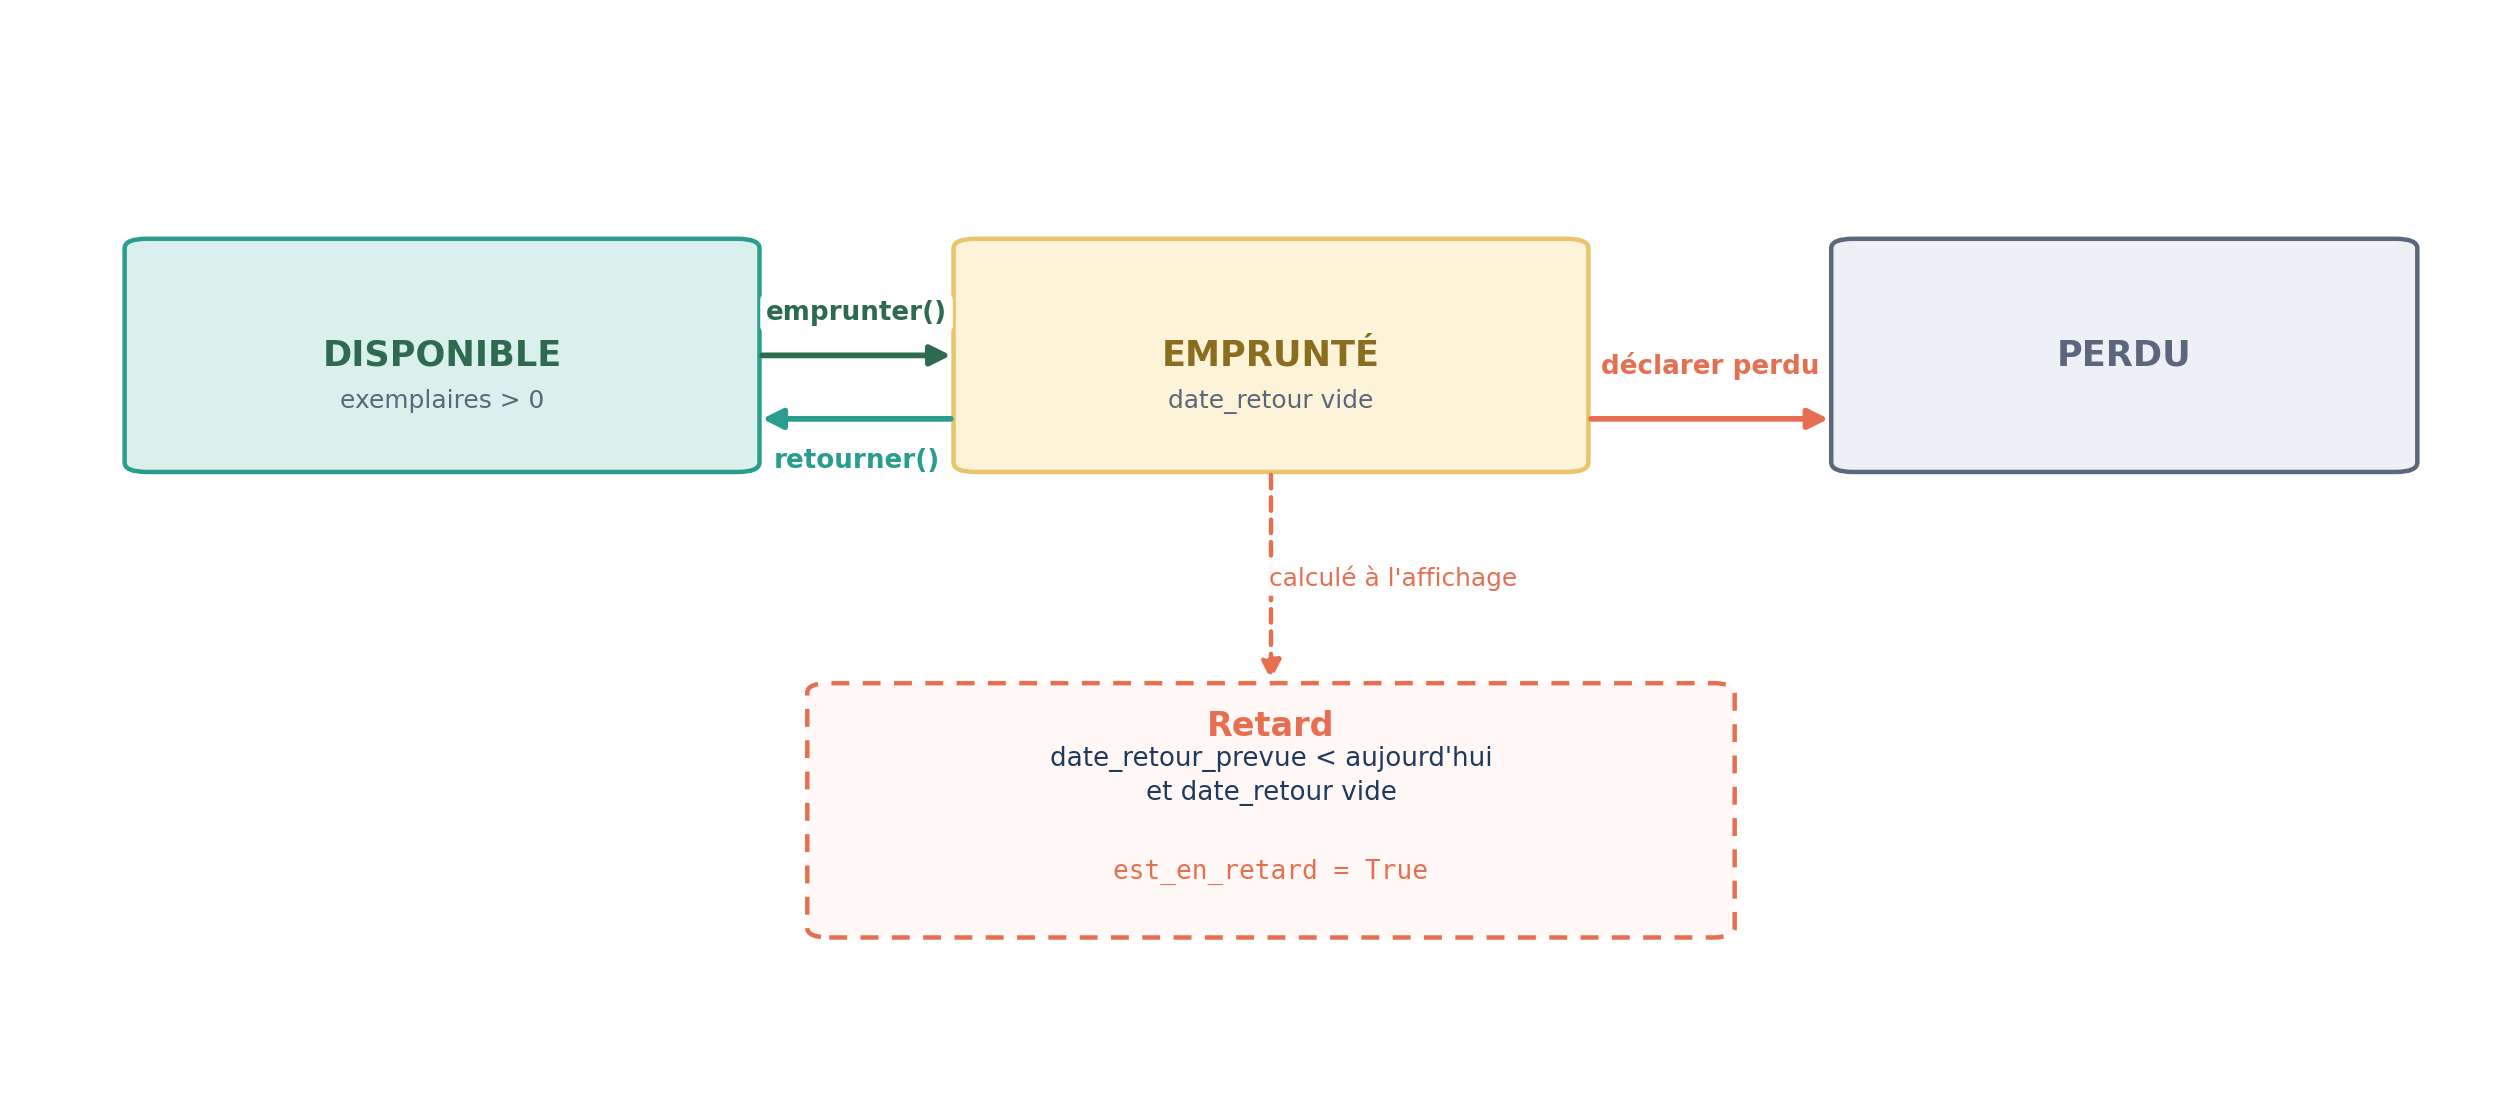
\includegraphics[width=0.92\textwidth]{images/cycle_emprunt.png}
\caption{Le cycle de vie d'un emprunt, de la demande au retour. Les règles de
validation protègent chaque transition.}
\label{fig:cycle-emprunt}
\end{figure}

\begin{codebox}[python]{catalogue/forms.py, extrait}
from django import forms
from django.utils import timezone

from .models import Emprunt


class EmpruntForm(forms.ModelForm):
    class Meta:
        model = Emprunt
        fields = ["livre", "membre", "date_retour_prevue", "remarque"]
        widgets = {
            "date_retour_prevue": forms.DateInput(attrs={"type": "date"}),
            "remarque": forms.Textarea(attrs={"rows": 3}),
        }

    def clean_date_retour_prevue(self):
        date_prevue = self.cleaned_data["date_retour_prevue"]
        if date_prevue < timezone.localdate():
            raise forms.ValidationError(
                "La date de retour ne peut pas être dans le passé."
            )
        return date_prevue

    def clean(self):
        donnees = super().clean()
        livre = donnees.get("livre")
        membre = donnees.get("membre")

        if livre and not livre.est_disponible:
            self.add_error(
                "livre",
                "Ce livre n'est pas disponible pour le moment.",
            )

        if membre and not membre.actif:
            self.add_error(
                "membre",
                "Ce membre est inactif et ne peut pas emprunter.",
            )

        if livre and membre:
            deja = Emprunt.objects.filter(
                livre=livre,
                membre=membre,
                date_retour__isnull=True,
            )
            if self.instance.pk:
                deja = deja.exclude(pk=self.instance.pk)
            if deja.exists():
                raise forms.ValidationError(
                    "Ce membre a déjà un emprunt en cours pour ce livre."
                )

        return donnees
\end{codebox}

\begin{description}[leftmargin=5.1cm,style=nextline]
  \item[\code{clean\_<champ>()}] Valide un champ précis. La valeur renvoyée remplace
  celle de \code{cleaned\_data}.
  \item[\code{clean()}] Validation globale, après les champs individuels.
  \item[\code{add\_error("champ", ...)}] Attache l'erreur au champ concerné.
  \item[\code{ValidationError}] Erreur générale, affichée dans
  \code{non\_field\_errors}.
\end{description}

\begin{bonne}
Les règles métier vont dans le formulaire ou dans le modèle, pas dans le gabarit.
Un formulaire peut être testé sans navigateur, avec
\code{EmpruntForm(data=...)}. C'est rapide et fiable.
\end{bonne}

\begin{piege}
Dans \code{clean()}, utilisez \code{donnees.get("livre")} et non
\code{donnees["livre"]}. Si le champ a déjà échoué, la clé est absente et vous
provoquez une \code{KeyError} au lieu d'afficher l'erreur principale.
\end{piege}

\subsection{La vue d'emprunt}

\begin{codebox}[python]{catalogue/views.py, extrait}
def emprunt_creer(request):
    if request.method == "POST":
        form = EmpruntForm(request.POST)
        if form.is_valid():
            emprunt = form.save()
            messages.success(
                request,
                f"Emprunt enregistré pour {emprunt.membre}.",
            )
            return redirect("catalogue:emprunt_liste")
    else:
        form = EmpruntForm()

    return render(
        request,
        "catalogue/emprunts/formulaire.html",
        {"form": form},
    )
\end{codebox}

\subsection{Enregistrer un retour}

Le retour n'est pas une modification libre : c'est une action datée.

\begin{codebox}[python]{catalogue/views.py, extrait}
from django.utils import timezone
from django.views.decorators.http import require_POST


@require_POST
def emprunt_retour(request, pk):
    emprunt = get_object_or_404(Emprunt, pk=pk)
    if emprunt.date_retour is None:
        emprunt.date_retour = timezone.localdate()
        emprunt.save(update_fields=["date_retour"])
        messages.success(request, "Le retour a été enregistré.")
    else:
        messages.info(request, "Ce livre a déjà été rendu.")
    return redirect("catalogue:emprunt_liste")
\end{codebox}

\begin{note}
\code{update\_fields} limite la requête \code{UPDATE} aux colonnes indiquées. C'est
plus rapide et cela évite d'écraser une modification concurrente sur un autre
champ. Utilisez-le quand vous modifiez un seul champ.
\end{note}

\section{Recherche et formulaire GET}

Un formulaire de recherche ne modifie rien : il utilise \code{GET}. Les paramètres
apparaissent dans l'URL, ce qui permet de partager un lien.

\begin{codebox}[python]{catalogue/forms.py, extrait}
class RechercheLivreForm(forms.Form):
    q = forms.CharField(
        required=False,
        label="Rechercher",
        widget=forms.TextInput(
            attrs={"type": "search", "placeholder": "Titre ou auteur"}
        ),
    )
    categorie = forms.ModelChoiceField(
        queryset=None,
        required=False,
        empty_label="Toutes les catégories",
    )
    tri = forms.ChoiceField(
        required=False,
        choices=[
            ("titre", "Titre"),
            ("recent", "Année décroissante"),
            ("auteur", "Auteur"),
        ],
    )

    def __init__(self, *args, **kwargs):
        super().__init__(*args, **kwargs)
        from .models import Categorie

        self.fields["categorie"].queryset = Categorie.objects.all()
\end{codebox}

\begin{attention}
Un \code{ModelChoiceField} exécute une requête pour construire ses options. Définir
le queryset dans \code{\_\_init\_\_} plutôt qu'au niveau de la classe évite une
requête au moment de l'import du module et permet de filtrer selon l'utilisateur.
\end{attention}

\begin{codebox}[python]{Vue avec formulaire GET}
def livre_liste(request):
    form = RechercheLivreForm(request.GET or None)
    livres = Livre.objects.select_related("auteur")

    if form.is_valid():
        mot = form.cleaned_data.get("q")
        categorie = form.cleaned_data.get("categorie")
        tri = form.cleaned_data.get("tri") or "titre"

        if mot:
            livres = livres.filter(titre__icontains=mot)
        if categorie:
            livres = livres.filter(categories=categorie)

        livres = livres.order_by(tri)

    return render(
        request,
        "catalogue/livres/liste.html",
        {"form": form, "livres": livres},
    )
\end{codebox}

\begin{note}
Avec \code{request.GET or None}, un premier appel sans paramètre donne
\code{None}, donc un formulaire non lié, sans erreurs. Un appel avec \code{?q=}
donne un formulaire lié, valide, avec une recherche vide. C'est le comportement
attendu.
\end{note}

\section{Les messages flash}

\begin{codebox}[python]{Les cinq niveaux}
from django.contrib import messages

messages.debug(request, "Détail technique.")
messages.info(request, "Information.")
messages.success(request, "Opération réussie.")
messages.warning(request, "Attention.")
messages.error(request, "Une erreur est survenue.")
\end{codebox}

Le partial \code{messages.html} créé au chapitre 3 les affiche. Les classes CSS
\code{success}, \code{error} et \code{warning} sont déjà prévues.

\begin{bonne}
Un message doit être court, au passé et actionnable : \og Le livre a été ajouté \fg,
pas \og Opération effectuée avec succès \fg. Évitez les messages techniques
(\code{IntegrityError}) visibles par l'utilisateur.
\end{bonne}

\section{Supprimer avec confirmation}

\begin{codebox}[python]{catalogue/views.py, extrait}
def livre_supprimer(request, slug):
    livre = get_object_or_404(Livre, slug=slug)

    if request.method == "POST":
        titre = livre.titre
        livre.delete()
        messages.success(request, f"Le livre « {titre} » a été supprimé.")
        return redirect("catalogue:livre_liste")

    return render(
        request,
        "catalogue/livres/supprimer.html",
        {"livre": livre},
    )
\end{codebox}

\begin{codebox}[html]{templates/catalogue/livres/supprimer.html}
{% extends "base.html" %}

{% block titre %}Supprimer {{ livre.titre }} | GesiBiblio{% endblock %}

{% block contenu %}
  <h1>Supprimer ce livre ?</h1>
  <p>
    Vous êtes sur le point de supprimer
    <strong>{{ livre.titre }}</strong>. Cette action est définitive.
  </p>

  <form method="post">
    {% csrf_token %}
    <button class="bouton bouton-danger" type="submit">
      Confirmer la suppression
    </button>
    <a class="bouton" href="{{ livre.get_absolute_url }}">Annuler</a>
  </form>
{% endblock %}
\end{codebox}

\begin{attention}
La suppression déclenche \code{on\_delete}. Avec \code{PROTECT}, Django refuse si
des emprunts existent. L'erreur remonte en \code{ProtectedError}. Attrapez-la pour
afficher un message clair au lieu d'une page 500.
\end{attention}

\begin{codebox}[python]{Gérer ProtectedError}
from django.db.models import ProtectedError

try:
    livre.delete()
except ProtectedError:
    messages.error(
        request,
        "Impossible de supprimer ce livre : des emprunts existent.",
    )
    return redirect(livre)
\end{codebox}

\section{Les vues génériques de formulaire}

Comme pour les listes, Django propose des classes.

\begin{codebox}[python]{catalogue/views.py, alternative CBV}
from django.urls import reverse_lazy
from django.views.generic import CreateView, DeleteView, UpdateView

from .forms import LivreForm
from .models import Livre


class LivreCreateView(CreateView):
    model = Livre
    form_class = LivreForm
    template_name = "catalogue/livres/formulaire.html"

    def get_context_data(self, **kwargs):
        contexte = super().get_context_data(**kwargs)
        contexte["titre_page"] = "Ajouter un livre"
        return contexte


class LivreUpdateView(UpdateView):
    model = Livre
    form_class = LivreForm
    template_name = "catalogue/livres/formulaire.html"


class LivreDeleteView(DeleteView):
    model = Livre
    template_name = "catalogue/livres/supprimer.html"
    success_url = reverse_lazy("catalogue:livre_liste")
\end{codebox}

\begin{description}[leftmargin=4.4cm,style=nextline]
  \item[\code{CreateView}] Affiche le formulaire en \code{GET}, enregistre en
  \code{POST} valide, puis redirige vers \code{get\_absolute\_url()}.
  \item[\code{UpdateView}] Même principe, avec un objet existant.
  \item[\code{DeleteView}] Affiche une confirmation en \code{GET}, supprime en
  \code{POST}.
  \item[\code{success\_url}] Utilise \code{reverse\_lazy} pour éviter un import
  circulaire.
\end{description}

\begin{piege}
\code{reverse\_lazy} est nécessaire dans un attribut de classe évalué à l'import.
\code{reverse} y serait exécuté trop tôt, avant que les URL ne soient chargées, et
provoquerait une \code{NoReverseMatch}.
\end{piege}

\section{Exercices}

\begin{exercice}[ : champ nombre de pages]
Ajoutez \code{nombre\_pages} au formulaire \code{LivreForm} et vérifiez qu'un
nombre négatif est refusé. Utilisez un \code{IntegerField} avec
\code{min\_value=0}.
\end{exercice}

\begin{correction}
Le modèle doit d'abord recevoir le champ, comme au chapitre 6. Puis, dans le
formulaire :

\begin{codebox}[python]{catalogue/forms.py, extrait}
nombre_pages = forms.IntegerField(
    min_value=0,
    required=False,
    label="Nombre de pages",
    help_text="Laissez vide si inconnu.",
)
\end{codebox}

Ajoutez \code{"nombre\_pages"} à \code{fields}. La validation refuse les valeurs
négatives avant même d'atteindre la base.
\end{correction}

\begin{exercice}[ : formulaire de contact complet]
Ajoutez un champ \code{sujet} avec trois choix : information, suggestion,
réclamation. Ajoutez une validation qui exige un message d'au moins vingt
caractères.
\end{exercice}

\begin{correction}
\begin{codebox}[python]{catalogue/forms.py, extrait}
class ContactForm(forms.Form):
    # ... champs existants
    sujet = forms.ChoiceField(
        choices=[
            ("information", "Information"),
            ("suggestion", "Suggestion"),
            ("reclamation", "Réclamation"),
        ],
        label="Sujet",
    )

    def clean_message(self):
        message = self.cleaned_data["message"]
        if len(message) < 20:
            raise forms.ValidationError(
                "Le message doit contenir au moins 20 caractères."
            )
        return message
\end{codebox}

L'erreur apparaît sous le champ \code{message}, pas dans les erreurs générales.
\end{correction}

\begin{exercice}[ : prolonger un emprunt]
Écrivez une vue \code{emprunt\_prolonger} qui ajoute quatorze jours à
\code{date\_retour\_prevue}, uniquement si l'emprunt n'est pas rendu et si le
membre est actif.
\end{exercice}

\begin{correction}
\begin{codebox}[python]{catalogue/views.py, extrait}
from datetime import timedelta

from django.views.decorators.http import require_POST


@require_POST
def emprunt_prolonger(request, pk):
    emprunt = get_object_or_404(Emprunt, pk=pk)

    if emprunt.date_retour is not None:
        messages.error(request, "Cet emprunt est déjà terminé.")
    elif not emprunt.membre.actif:
        messages.error(request, "Le membre est inactif.")
    else:
        emprunt.date_retour_prevue += timedelta(days=14)
        emprunt.save(update_fields=["date_retour_prevue"])
        messages.success(request, "L'emprunt a été prolongé de 14 jours.")

    return redirect("catalogue:emprunt_liste")
\end{codebox}

\code{timedelta(days=14)} ajoute quatorze jours à une date. La vue est protégée
par \code{require\_POST} : la prolongation ne peut pas être déclenchée par un lien.
\end{correction}

\begin{retenir}
\begin{itemize}
  \item Un formulaire Django génère, valide et nettoie les données.
  \item \code{ModelForm} évite de répéter les champs du modèle.
  \item \code{request.FILES} et \code{enctype} sont obligatoires pour un fichier.
  \item \code{clean\_<champ>()} valide un champ, \code{clean()} valide l'ensemble.
  \item \code{commit=False} permet d'ajouter une valeur avant l'enregistrement.
  \item Après un \code{POST} réussi, redirigez pour éviter le double envoi.
  \item \code{CreateView}, \code{UpdateView} et \code{DeleteView} sont des
        alternatives concises aux vues fonction.
\end{itemize}
\end{retenir}
